%% abtex2-modelo-trabalho-academico.tex, v-1.9.7 laurocesar
%% Copyright 2012-2018 by abnTeX2 group at http://www.abntex.net.br/ 
%%
%% This work may be distributed and/or modified under the
%% conditions of the LaTeX Project Public License, either version 1.3
%% of this license or (at your option) any later version.
%% The latest version of this license is in
%%   http://www.latex-project.org/lppl.txt
%% and version 1.3 or later is part of all distributions of LaTeX
%% version 2005/12/01 or later.
%%
%% This work has the LPPL maintenance status `maintained'.
%% 
%% The Current Maintainer of this work is the abnTeX2 team, led
%% by Lauro César Araujo. Further information are available on 
%% http://www.abntex.net.br/
%%
%% This work consists of the files abntex2-modelo-trabalho-academico.tex,
%% abntex2-modelo-include-comandos and abntex2-modelo-references.bib
%%

% ------------------------------------------------------------------------
% ------------------------------------------------------------------------
% abnTeX2: Modelo de Trabalho Academico (tese de doutorado, dissertacao de
% mestrado e trabalhos monograficos em geral) em conformidade com 
% ABNT NBR 14724:2011: Informacao e documentacao - Trabalhos academicos -
% Apresentacao
% ------------------------------------------------------------------------
% ------------------------------------------------------------------------

\documentclass[
	% -- opções da classe memoir --
	12pt,				% tamanho da fonte
	openany,			% capítulos começam em pág ímpar (insere página vazia caso preciso)
	twoside,			% para impressão em recto e verso. Oposto a oneside
	a4paper,			% tamanho do papel. 
	% -- opções da classe abntex2 --
	%chapter=TITLE,		% títulos de capítulos convertidos em letras maiúsculas
	%section=TITLE,		% títulos de seções convertidos em letras maiúsculas
	%subsection=TITLE,	% títulos de subseções convertidos em letras maiúsculas
	%subsubsection=TITLE,% títulos de subsubseções convertidos em letras maiúsculas
	% -- opções do pacote babel --
	english,			% idioma adicional para hifenização
	brazil				% o último idioma é o principal do documento
	]{abntex2}

% ---
% Pacotes básicos 
% ---
\usepackage{lmodern}			% Usa a fonte Latin Modern			
\usepackage[T1]{fontenc}		% Selecao de codigos de fonte.
\usepackage[utf8]{inputenc}		% Codificacao do documento (conversão automática dos acentos)
\usepackage{indentfirst}		% Indenta o primeiro parágrafo de cada seção.
\usepackage{color}				% Controle das cores
\usepackage{graphicx}			% Inclusão de gráficos
\usepackage{microtype} 			% para melhorias de justificação
\usepackage{placeins}


% ---
		
% ---
% Pacotes adicionais, usados apenas no âmbito do Modelo Canônico do abnteX2
% ---
\usepackage{lipsum}				% para geração de dummy text
% ---

% ---
% Pacotes de citações
% ---
\usepackage[brazilian,hyperpageref]{backref}	 % Paginas com as citações na bibl
\usepackage[alf]{abntex2cite}	% Citações padrão ABNT
\usepackage{hyperref}
\usepackage{xurl} % quebra URLs longas automaticamente
% --- 
% CONFIGURAÇÕES DE PACOTES
% --- 

% ---
% Configurações do pacote backref
% Usado sem a opção hyperpageref de backref
\renewcommand{\backrefpagesname}{Citado na(s) página(s):~}
% Texto padrão antes do número das páginas
\renewcommand{\backref}{}
% Define os textos da citação
\renewcommand*{\backrefalt}[4]{
	\ifcase #1 %
		Nenhuma citação no texto.%
	\or
		Citado na página #2.%
	\else
		Citado #1 vezes nas páginas #2.%
	\fi}%
% ---

% ---
% Informações de dados para CAPA e FOLHA DE ROSTO
% ---
\titulo{VIP PENHA}
\autor{
  {\large IFSP - Instituto Federal de Educação, Ciência e Tecnologia} \\
  {\large Câmpus São Paulo} \\[1cm]
  \makebox[0.60\textwidth][l]{BEATRIZ MUNIZ DE BARROS} \makebox[0.20\textwidth][r]{SP3161315}\\
  \makebox[0.60\textwidth][l]{GEAN CARLOS DE SOUSA BANDEIRA} \makebox[0.20\textwidth][r]{SP3030075}\\
  \makebox[0.60\textwidth][l]{KHALIL KHALID ABOU ANCHE} \makebox[0.20\textwidth][r]{SP3121925}\\
  \makebox[0.60\textwidth][l]{MARCELO FLORES VALDEZ} \makebox[0.20\textwidth][r]{SP3039056}\\
  \makebox[0.60\textwidth][l]{MATHEUS PRANDO APPOLINARIO BARBOSA} \makebox[0.20\textwidth][r]{SP3121747}\\
  \makebox[0.60\textwidth][l]{RAFAEL VALVERDE ZANATA DA SILVA} \makebox[0.20\textwidth][r]{SP3119866}\\
  \makebox[0.60\textwidth][l]{VITOR DA SILVA OLIVEIRA} \makebox[0.20\textwidth][r]{SP3020589}\\
}


\local{São Paulo - SP - Brasil}
\data{2025}
\orientador{Marcelo Tavares de Santana}
\instituicao{
  IFSP - Instituto Federal de Educação, Ciência e Tecnologia \\
  Câmpus São Paulo \\
  Tecnologia em Análise e Desenvolvimento de Sistemas
}
\tipotrabalho{Projeto Integrado I}
\preambulo{
 Projeto desenvolvido como parte das atividades da disciplina Projeto Integrado, apresentado ao Instituto Federal de Educação, Ciência e Tecnologia de São Paulo, Câmpus São Paulo, curso de Tecnologia em Análise e Desenvolvimento de Sistemas.
}
% ---


% ---
% Configurações de aparência do PDF final

% alterando o aspecto da cor azul
\definecolor{blue}{RGB}{41,5,195}

% informações do PDF
\makeatletter
\hypersetup{
     	%pagebackref=true,
		pdftitle={\@title}, 
		pdfauthor={\@author},
    	pdfsubject={\imprimirpreambulo},
	    pdfcreator={LaTeX with abnTeX2},
		pdfkeywords={abnt}{latex}{abntex}{abntex2}{trabalho acadêmico}, 
		colorlinks=true,       		% false: boxed links; true: colored links
    	linkcolor=blue,          	% color of internal links
    	citecolor=blue,        		% color of links to bibliography
    	filecolor=magenta,      		% color of file links
		urlcolor=blue,
		bookmarksdepth=4
}
\makeatother
% --- 

% ---
% Posiciona figuras e tabelas no topo da página quando adicionadas sozinhas
% em um página em branco. Ver https://github.com/abntex/abntex2/issues/170
\makeatletter
\setlength{\@fptop}{5pt} % Set distance from top of page to first float
\makeatother
% ---

% ---
% Possibilita criação de Quadros e Lista de quadros.
% Ver https://github.com/abntex/abntex2/issues/176
%
\newcommand{\quadroname}{Quadro}
\newcommand{\listofquadrosname}{Lista de quadros}

\newfloat[chapter]{quadro}{loq}{\quadroname}
\newlistof{listofquadros}{loq}{\listofquadrosname}
\newlistentry{quadro}{loq}{0}

% configurações para atender às regras da ABNT
\setfloatadjustment{quadro}{\centering}
\counterwithout{quadro}{chapter}
\renewcommand{\cftquadroname}{\quadroname\space} 
\renewcommand*{\cftquadroaftersnum}{\hfill--\hfill}

\setfloatlocations{quadro}{hbtp} % Ver https://github.com/abntex/abntex2/issues/176

% Evitar página em branco após o resumo
\let\oldcleardoublepage\cleardoublepage
\let\cleardoublepage\clearpage
% ---

% --- 
% Espaçamentos entre linhas e parágrafos 
% --- 

% O tamanho do parágrafo é dado por:
\setlength{\parindent}{1.3cm}

% Controle do espaçamento entre um parágrafo e outro:
\setlength{\parskip}{0.2cm}  % tente também \onelineskip

% ---
% compila o indice
% ---
\makeindex
% ---

% ----
% Início do documento
% ----
\begin{document}

% Seleciona o idioma do documento (conforme pacotes do babel)
%\selectlanguage{english}
\selectlanguage{brazil}

% Retira espaço extra obsoleto entre as frases.
\frenchspacing 

% ----------------------------------------------------------
% ELEMENTOS PRÉ-TEXTUAIS
% ----------------------------------------------------------
% \pretextual

% ---
% Capa
% ---



% ---

% ---
% Folha de rosto
% (o * indica que haverá a ficha bibliográfica)
\begin{capa}

  \begin{center}
    {\ABNTEXchapterfont\large\imprimirautor}

    \vspace*{\fill}\vspace*{\fill}
    \begin{center}
      \ABNTEXchapterfont\bfseries\Large\imprimirtitulo
    \end{center}
    \vspace*{\fill}
    
    \hspace{.45\textwidth}
    \begin{minipage}{.5\textwidth}
    \end{minipage}%

    \vspace*{1.5cm} % Aumenta o espaço após o preâmbulo

    \vspace*{0.8cm} % Diminui o espaço antes da data

  \end{center}

  \begin{center}
    {\large\imprimirlocal}
    \par
    {\large\imprimirdata}
  \end{center}

\end{capa}

\begin{folhadeaprovacao}

  \begin{center}
    {\ABNTEXchapterfont\large\imprimirautor}

    \vspace*{\fill}\vspace*{\fill}
    \begin{center}
      \ABNTEXchapterfont\bfseries\Large\imprimirtitulo
    \end{center}
    \vspace*{\fill}
    
    \hspace{.45\textwidth}
    \begin{minipage}{.5\textwidth}
        \imprimirpreambulo
    \end{minipage}%

    \vspace*{1.5cm} % Aumenta o espaço após o preâmbulo

    \begin{center}
        IFSP - Instituto Federal de Educação, Ciência e Tecnologia \\
        Câmpus São Paulo \\
        Tecnologia em Análise e Desenvolvimento de Sistemas
    \end{center}

    \vspace*{0.8cm} % Diminui o espaço antes da data

  \end{center}

  \begin{center}
    {\large\imprimirlocal}
    \par
    {\large\imprimirdata}
  \end{center}

\end{folhadeaprovacao}

% ---

% ---
% Dedicatória
% ---

% ---


% ---
% RESUMOS
% ---


% resumo em português

\setlength{\absparsep}{18pt} % ajusta o espaçamento dos parágrafos do resumo
\begin{resumo}
Este projeto descreve a criação de um sistema de controle de estoque para a loja de eletrônicos VIP PENHA. Em um cenário de rápido avanço tecnológico e crescente competitividade de mercado, a gestão eficiente de recursos é essencial para empreendimentos. O sistema foi desenvolvido para otimizar o controle de produtos, tornando a operação mais eficiente. 

A problemática central é a falta de controle de estoque e os erros de processos manuais na "VIP PENHA". A solução implementada é um sistema unificado que permite o cadastro de produtos, o controle de entradas e saídas de mercadorias, e a geração automática de relatórios gerenciais. Isso resultou na redução de erros manuais, na diminuição do tempo gasto na gestão do estoque e na melhoria da tomada de decisões estratégicas, oferecendo uma perspectiva clara sobre o desempenho do inventário. 

Para o desenvolvimento do sistema, foram realizadas pesquisas sobre gestão de estoque e sistemas de informação, utilizando uma metodologia de trabalho ágil, o Kanban. O projeto abrangeu o detalhamento de funcionalidades, requisitos técnicos, arquitetura do sistema (front-end, back-end, banco de dados e infraestrutura), tecnologias empregadas, planos de testes e planejamentos financeiros.


 \textbf{Palavras-chave}: Sistema de estoque. Gestão de produtos. Automação. Relatórios gerenciais. Kanban. 
\end{resumo}

% resumo em inglês
\begin{resumo}[Abstract]
 \begin{otherlanguage*}{english}
This project describes the creation of an inventory control system for the VIP PENHA electronics store. In a scenario of rapid technological advancement and increasing market competitiveness, efficient resource management is essential for businesses. The system was developed to
optimize product control, making operations more efficient. 

The central problem addressed is the lack of inventory control and manual process errors at "VIP PENHA". The implemented solution is a unified system that allows product registration, control of goods entry and exit, and automatic generation of management reports. This resulted in the reduction of manual errors, decreased time spent on inventory management, and improved strategic decision-making, offering a clear perspective on inventory performance. 

For the system's development, research on inventory management and information systems was conducted, utilizing an agilemethodology, Kanban. The project covered the detailing of functionalities, technical requirements, system architecture (front-end, back-end, database, and infrastructure), technologies employed, test plans, and financial planning.


   \vspace{\onelineskip}
 
   \noindent 
   \textbf{Keywords}: Inventory management system. Product management. Automation. Management reports. Kanban.
 \end{otherlanguage*}
\end{resumo}


% ---

% ---
% inserir lista de ilustrações
% ---
\pdfbookmark[0]{\listfigurename}{lof}
\listoffigures*
\clearpage
% ---

% ---
% inserir lista de quadros
% ---
\pdfbookmark[0]{\listofquadrosname}{loq}
\listofquadros*
\cleardoublepage
% ---

% ---
% inserir lista de tabelas
% ---
\pdfbookmark[0]{\listtablename}{lot}
\listoftables*
\cleardoublepage
% ---

% --
% inserir lista de símbolos
% ---

% ---

% ---
% inserir o sumario
% ---
\pdfbookmark[0]{\contentsname}{toc}
\tableofcontents*
\cleardoublepage
% ---



% ----------------------------------------------------------
% ELEMENTOS TEXTUAIS
% ----------------------------------------------------------
\textual

% ----------------------------------------------------------
% Introdução (exemplo de capítulo sem numeração, mas presente no Sumário)
% ----------------------------------------------------------
\chapter{Introdução}
% ----------------------------------------------------------

Na época atual, de rápido avanço tecnológico, onde a competitividade no mercado só vem aumentando, a gestão eficiente dos recursos tornou-se um fator determinante para o sucesso de empreendimentos, seja de pequeno, médio e grande porte. Pensando nisso, o projeto consiste no desenvolvimento de um sistema de gerenciamento de estoque voltado para a loja de artigos eletrônicos VIP PENHA.

Diante das transformações que vêm ocorrendo no ambiente corporativo, especialmente com o avanço contínuo das tecnologias, torna-se urgente que as empresas que ainda não iniciaram esse processo comecem a repensar suas práticas. Adotar ferramentas digitais é fundamental não só para garantir a segurança dos processos internos e uma operação mais estruturada, mas também para assegurar que o negócio consiga acompanhar as exigências do mercado atual e preserve sua relevância diante da concorrência. A integração tecnológica proporciona maior agilidade operacional, embasa decisões estratégicas com dados e minimiza falhas, tornando-se um grande diferencial competitivo. Segundo  \citeonline{laudon2014} , os sistemas da informação são a base para conduzir os negócios na era atual, onde as empresas utilizam os sistemas para atingir a excelência operacional, novos produtos, serviços e negócios. Diante desse cenário, um bom sistema de gerenciamento providenciará a ajuda necessária para o crescimento e expansão da loja.

Além disso, considerando o contexto específico da gestão de estoque, a adoção de ferramentas tecnológicas exerce um papel fundamental na administração das operações logísticas, ao garantir mais controle e visibilidade do fluxo das entradas e saídas dos produtos. Também reduz drasticamente os erros operacionais, perda de informações, além de permitir um planejamento mais eficiente dos recursos. Tendo os dados precisos e atualizados constantemente, é possível realizar análises extremamente precisas em todos os setores, como a reposição, o armazenamento e as movimentações dos produtos.

Posto isso, fica claro, portanto, que a digitalização deixou de ser opcional e passou a representar um pilar estratégico para empresas que buscam eficiência, segurança e competitividade. No contexto de gestão de estoque, incorporar tecnologias possibilita controles mais precisos e decisões mais embasadas. Diante de um cenário empresarial cada vez mais influenciado pelos dados e pela agilidade, investir na transformação digital se faz essencial para garantir a sustentabilidade e o crescimento da organização.


\section{Objetivos}

Nesta seção serão apresentados os objetivos do projeto, ele estão divididos em objetivo geral e objetivos específicos. O objetivo geral descreve a meta principal do projeto, já os objetivos específicos descrevem as etapas e funcionalidades para o alcance da meta final.

\subsection{Objetivo Geral}

Desenvolver um sistema de gerenciamento de estoque para a loja VIP PENHA, visando transformar a gestão de inventário em um processo automatizado e estratégico. O sistema irá otimizar o controle de produtos, diminuir erros manuais e reduzir o tempo gasto na gestão, ao possibilitar o cadastro detalhado de itens, o monitoramento de entradas e saídas em tempo real e a configuração de alertas de estoque mínimo. 

\subsection{Objetivos Específicos}

\begin{itemize}
    \item Desenvolver uma plataforma de cadastro de produtos, permitindo o registro e atualização dos produtos no estoque.
    \item Permitir a análise do desempenho do estoque por meio da automatização de relatórios gerenciais, identificando produtos mais vendidos, vendas realizadas e necessidades de reposição.
    \item Reduzir os erros manuais ao implementar processos automatizados.
\end{itemize}

\section{Problema e Solução Proposta}

Nessa seção serão apresentados os problemas enfrentados pela loja VIP PENHA em relação ao gerenciamento do seu estoque, assim como a solução proposta para resolver esses problemas. A seguir, são descritos os principais desafios e como o sistema visa solucioná-los de maneira eficiente.

\subsection{Problema}

Devido a recentes expansões, a loja VIP PENHA vem enfrentando problemas como a falta de controle do seu estoque devido a ausência de um sistema automatizado. Essa lacuna tem gerado uma série de complicações que comprometem o funcionamento eficiente da loja. A principal delas é a falta de controle em tempo real das mercadorias, dificultando o acompanhamento preciso da quantidade de produtos disponíveis e resultando em faltas ou excessos de estoque.

Além disso, o processo manual de registro das entradas e saídas de produtos tem sido fonte constante de erros, como registros duplicados, extravios e divergências entre o estoque físico e o registrado. A inexistência de relatórios gerenciais confiáveis impede uma análise clara do desempenho da loja, dificultando a tomada de decisões estratégicas.

Outro ponto preocupante é a falta de rastreabilidade do histórico de movimentações dos produtos, o que inviabiliza a realização de auditorias e a identificação de padrões de consumo. Além disso, a ausência de integração entre os setores de compras, vendas e estoque gera desorganização e atrasos operacionais. Todos esses fatores combinados impactam negativamente a eficiência, o atendimento ao cliente e o potencial de crescimento da loja.


\subsection{Solução Proposta}

Para resolver esses problemas, propõe-se o desenvolvimento de um sistema de gerenciamento de estoque voltado às necessidades específicas da loja VIP PENHA. A implementação desse sistema permitirá centralizar e automatizar os principais processos envolvidos no controle de mercadorias, trazendo mais eficiência, organização e confiabilidade às operações da empresa.

O sistema contará com funcionalidades essenciais como o cadastro de produtos, controle automatizado das entradas e saídas de mercadorias e geração de relatórios gerenciais. Com isso, será possível acompanhar em tempo real o status do estoque, identificar rapidamente produtos em falta ou com excesso, e tomar decisões mais claramente com base nos relatórios fornecidos pelo sistema.

Diferente das soluções genéricas disponíveis no mercado, o sistema VIP PENHA será totalmente adaptado à realidade e ao fluxo de trabalho da loja, oferecendo uma interface simples, intuitiva e de fácil uso. Além disso, o sistema terá baixo custo de implementação e manutenção, tornando-se uma alternativa acessível e eficiente para pequenos comércios que desejam modernizar sua gestão de estoque sem recorrer a plataformas complexas e de alto custo.

Com a adoção dessa solução, a loja VIP PENHA poderá reduzir drasticamente os erros operacionais, melhorar o fluxo de trabalho, aumentar a produtividade da equipe e oferecer um atendimento mais ágil e eficiente aos clientes. Dessa forma, o sistema contribuirá significativamente para o crescimento sustentável e a consolidação da loja no mercado.
 

\section{Justificativa}
Atualmente, para uma empresa, ter um sistema digitalizado para a gestão de estoque é uma questão de sobrevivência. Para entender melhor esse panorama, é importante observar o estágio em que se encontram os pequenos negócios no Brasil, e sendo assim, compreender o nível de maturidade digital das empresas brasileiras é de grande relevância. 

Segundo o estudo Mapa de Digitalização das Micro e Pequenas Empresas Brasileiras de 2024, desenvolvido pela Fundação Getulio Vargas (FGV) em parceria com a  \citeonline{ABDIMaturidade2024}, o índice médio de maturidade digital dos pequenos negócios é de 35 pontos, em uma escala de 0 a 80, indicando um nível de 43,75\% de maturidade média. A pesquisa aponta também que apenas 27\% das empresas possuem um sistema de gestão que integra as bases de dados de todas as áreas do negócio . 

Nesse cenário, a implementação de um sistema de gestão digital na loja VIP PENHA representa uma ação estratégica, não apenas para acompanhar a modernização do mercado, mas principalmente para solucionar gargalos que hoje prejudicam o desempenho e o crescimento do negócio.

Além disso, sistemas digitais de gestão de estoque oferecem vantagens claras, como:

\begin{itemize}
    \item \textbf{Redução de erros operacionais:} O sistema eliminará divergências entre o estoque físico e o digital, garantindo registros precisos e confiáveis.
    \item \textbf{Acompanhamento do sistema:} Com dados digitalizados, é possível acompanhar todas as movimentações de entradas e saídas de produtos com uma extrema facilidade e confiabilidade.
    \item \textbf{Agilidade nos processos:} As movimentações de produtos serão registradas com mais velocidade e precisão, reduzindo o tempo gasto com conferências e atualizações manuais.
    \item \textbf{Otimização de recursos:} Com um sistema de gerênciamento tecnológico, é possível fazer uma melhor utilização do espaço físico disponível, além de um melhor controle dos recursos financeiros, evitando o excesso e a falta de produtos.
    \item \textbf{Geração de relatórios:} As informações poderão ser analisadas rapidamente por meio de relatórios personalizados, auxiliando na tomada de decisões estratégicas.
\end{itemize}

Digitalizar o sistema de estoque é, portanto, um passo essencial para empresas que desejam crescer de forma organizada, segura e competitiva. Ao automatizar esse setor, os gestores têm mais controle e previsibilidade, elementos indispensáveis para a sobrevivência e sustentabilidade de qualquer negócio, especialmente no cenário atual de constantes mudanças e demandas cada vez mais dinâmicas.

\section{Análise de Concorrência}

Nesta seção, foi realizada uma análise dos principais sistemas de gerenciamento de estoque disponíveis no mercado, com foco em soluções utilizadas por lojas de pequeno e médio porte. Assim, demostrando quais as vantagens de usar o sistema que produzimos.

\subsection{Concorrente 1: Bling ERP}
O Bling é um sistema ERP completo que oferece controle de estoque, vendas, emissão de notas fiscais e integração com plataformas de e-commerce. É bastante utilizado por empresas que também vendem online, oferecendo funcionalidades robustas. No entanto, seu uso pode ser complexo para iniciantes, além de exigir pagamento mensal.

\subsection{Concorrente 2: Tiny ERP}
O Tiny ERP oferece funcionalidades similares ao Bling, como controle de estoque, pedidos, emissão de notas fiscais e integração com o setor financeiro. É conhecido por sua interface amigável, mas ainda assim exige uma curva de aprendizado e também é um serviço pago.

\subsection{Concorrente 3: Nex}
O Nex é um sistema gratuito e simples, ideal para pequenos comércios. Permite o cadastro de produtos, controle de estoque e de vendas. É bastante intuitivo, mas possui limitações em relação à integração com outras plataformas e funcionalidades avançadas.

\subsection{Concorrente 4: MarketUP}
O MarketUP é uma solução gratuita e bastante completa, oferecendo controle de estoque, vendas, financeiro e emissão de notas fiscais. No entanto, a interface pode ser confusa, especialmente para usuários menos experientes, e o suporte técnico é limitado.

\subsection{Quatro Comparativo}

\begin{quadro}[htb]
\caption{\label{quadro_comparativo}Comparação entre Sistemas de Gerenciamento de Estoque}
\begin{tabular}{|p{3.2cm}|p{5.5cm}|p{2.2cm}|p{4.1cm}|}
\hline
\textbf{Sistema} & \textbf{Funcionalidades Principais} & \textbf{Preço} & \textbf{Observações} \\
\hline
\textbf{Bling ERP} & Controle de estoque, vendas, emissão de notas fiscais, integração com e-commerce & Pago & Funcional, mas complexo para iniciantes \\
\hline
\textbf{Tiny ERP} & Estoque, pedidos, notas fiscais, controle financeiro & Pago & Interface moderna, porém exige curva de aprendizado \\
\hline
\textbf{Nex} & Cadastro de produtos, estoque e vendas & Gratuito & Intuitivo, ideal para pequenos comércios, porém limitado \\
\hline
\textbf{MarketUP} & Estoque, vendas, financeiro, notas fiscais & Gratuito & Completo, mas com interface confusa e suporte limitado \\
\hline
\textbf{"Sistema VIP PENHA} & Controle de estoque em tempo real, alerta de estoque mínimo, cadastro técnico de produtos, controle de garantias e geração de relatórios personalizados & Gratuito/Personalizado & Sistema desenvolvido especificamente para a realidade da loja VIP PENHA, com interface simples e fácil aprendizado, garantindo maior eficiência e redução de erros. \\
\hline
\end{tabular}
\end{quadro}

% ---
% Capitulo com exemplos de comandos inseridos de arquivo externo 
% ---
\include{abntex2-modelo-include-comandos}
% ---

\chapter{Revisão da Literatura}
O presente capítulo tem como objetivo apresentar estudos, teorias e contribuições acadêmicas relacionados à gestão de estoque em empresas.
\section{Histórico do Gerenciamento de Estoque}
A gestão de estoque é uma prática que acompanha a humanidade há milênios, realizar uma armazenagem inteligente dos recursos se mostrou essencial para a raça humana desde o seu primórdio. Um exemplo é o Período Uruk, nele foram desenvolvidas várias técnicas de gestão, como o uso de imagens e símbolos para administrar a estocagem de grãos, frutas e produtos, o que impulsionou essa sociedade a grandes avanços e ao desenvolvimento de um dos primeiros sistemas de escrita da história. \cite{Albright1996}

Durante a revolução industrial, com a produção em larga escala, houve um grande aumento na necessidade de melhores práticas de gerenciamento de estoque. O aumento da demanda de abastecimento contínuo do mercado levou ao desenvolvimento de melhores técnicas de controle e armazenamento dos produtos. \cite{DIAS2021}

Em meados do século XX, com o avanço da computação e o surgimento de sistemas informatizados, houve uma verdadeira revolução na gestão de estoque. O uso de softwares para a administração como o Material Requirements Planning (MRP), desenvolvido na década de 1960, e posteriormente o Enterprise Resource Planning (ERP), introduzido nos anos 1990, criando uma nova era na administração de estoque com o uso de dados e automação de processos.

Dessa forma, o percurso histórico ressalta a complexidade e a necessidade de soluções de gestão de estoque modernas, capazes de integrar processos e informações de maneira eficiente. A evolução dos métodos, desde o controle manual até os sistemas ERP, demonstra que a tecnologia tornou-se essencial para a administração eficaz dos estoques. No entanto, também evidencia que muitas das soluções existentes no mercado não são adequadas à realidade de pequenos comércios, por demandarem altos investimentos e infraestrutura avançada.

Sendo assim, o desenvolvimento do sistema proposto para a VIP PENHA se apoia nesse entendimento histórico e tecnológico: trata-se de uma solução digital sob medida, que busca aliar os princípios da gestão moderna, precisão, integração e automação e às necessidades práticas de um negócio local. 

\section{Atualidades do Gerenciamento de Estoque}
Atualmente, o processo de gerência de estoque encontra-se em níveis muito altos de integração tecnológica, com várias ferramentas modernas sendo aliadas nessa importante tarefa. A utilização de sistemas automatizados, softwares de gestão integrada (ERP) e tecnologias de rastreamento têm sido amplamente adotadas pelas empresas com o objetivo de melhorar o controle, a acuracidade e a eficiência do estoque.

Em resumo, uma administração de estoque correta e moderna deve ter seus alicerces inseridos na tecnologia e em soluções que integrem os processos físicos aos sistemas digitais da empresa. Essas ferramentas contribuem para reduzir falhas humanas, otimizar recursos e fortalecer a capacidade competitiva das organizações. Diante desse cenário, é esperado que a transformação digital continue a evoluir e a redefinir o papel do gerenciamento de estoque, tornando-o cada vez mais estratégico para o sucesso empresarial.

\chapter{Gestão do Projeto}

Este capítulo apresenta como a equipe foi estruturada, quais papéis e responsabilidades cada membro assumiu, além da metodologia de gerenciamento adotada ao longo do desenvolvimento. Também são descritas as ferramentas utilizadas para organização das tarefas e o repositório da aplicação.

\section{Organização da Equipe}

A equipe do projeto foi composta por membros com múltiplas atribuições, de modo a garantir flexibilidade e colaboração entre as diferentes áreas de desenvolvimento, testes e gestão. Abaixo, a distribuição de funções e responsabilidades:

\begin{table}[htbp] 
\centering
\begin{tabular}{|l|l|}
\hline
\textbf{Membro} & \textbf{Função(ões)} \\ \hline
Vitor           & Gestor, DBA           \\ \hline
Matheus         & DBA, Back-end         \\ \hline
Beatriz         & Front-end, Back-end   \\ \hline
Rafael          & Front-end, QA         \\ \hline
Khalil              & Back-end, QA          \\ \hline
Gean            & QA                    \\ \hline
Marcelo         & Front-end, QA         \\ \hline
\end{tabular}
\caption{Composição da equipe e funções}
\end{table}


\subsection{Responsabilidades/Papéis}

Os papéis desempenhados pela equipe foram definidos com base em suas competências e nas necessidades do projeto. A seguir, os principais papéis e suas responsabilidades:

\begin{itemize}
    \item \textbf{Gestor}: Responsável pelo planejamento, organização, acompanhamento das atividades, definição de cronogramas e mediação da comunicação interna e externa.
    \item \textbf{DBA (Administrador de Banco de Dados)}: Responsável pela modelagem do banco de dados, criação e manutenção das estruturas de dados, performance e integridade das informações.
    \item \textbf{Desenvolvedor Back-end}: Responsável pela implementação da lógica de negócio, criação de APIs, segurança e integração com o banco de dados.
    \item \textbf{Desenvolvedor Front-end}: Responsável pela criação da interface visual da aplicação, usabilidade, responsividade e interação com o usuário.
    \item \textbf{QA (Quality Assurance)}: Responsável pela garantia da qualidade da aplicação, planejamento e execução de testes funcionais, validação dos requisitos e registro de bugs.
\end{itemize}

\section{Metodologia de Gestão}

\subsection{Kanban}

A equipe optou pela utilização do método \textbf{Kanban} para o gerenciamento das atividades do projeto. Essa metodologia permite o acompanhamento visual focando na entrega contínua e em tempo real das tarefas.Add commentMore actions

O quadro Kanban utilizado possui as seguintes colunas:

\begin{itemize}
    \item \textbf{Backlog – Código:} Armazena ideias e funcionalidades relacionadas à implementação do código que ainda não foram iniciadas.
    \item \textbf{Backlog – Documentação:} Armazena tarefas de documentação que ainda não foram iniciadas.
    \item \textbf{Design:} Etapa dedicada à elaboração de pesquisas.
    \item \textbf{A Fazer:} Tarefas já priorizadas e planejadas, aguardando início.
    \item \textbf{Em Andamento:} Tarefas em desenvolvimento.
    \item \textbf{Revisão de Código:} Etapa de verificação e revisão do código antes da finalização.
    \item \textbf{Fase de Teste:} Validação e testes das funcionalidades desenvolvidas.
    \item \textbf{Concluído:} Tarefas finalizadas, revisadas e testadas com sucesso.
\end{itemize}

As atividades são constantemente avaliadas e realocadas entre as colunas conforme seu progresso, promovendo transparência e melhoria contínua do fluxo de trabalho.

\subsection{Funções da Equipe no Kanban}

A seguir, serão apresentadas as funções da equipe no projeto, com os respectivos membros atribuídos e as responsabilidades de cada papel:

\begin{table}[htbp]
\centering
\begin{tabular}{|l|l|l|}
\hline
\textbf{PO} & \textbf{Flow manager} & \textbf{Team Member} \\ \hline
Vitor        & Beatriz      & Matheus             \\ \hline
             &              & Khalil         \\ \hline
             &              & Gean                \\ \hline
             &              & Marcelo             \\ \hline
             &              & Rafael              \\ \hline
\end{tabular}
\caption{Funções da Equipe}
\end{table}

\FloatBarrier

\subsection{Responsabilidades de cada papel}

\begin{itemize}
    \item \textbf{PO (Product Owner)}: 
    Responsável por representar os interesses do cliente e das partes interessadas. No contexto Kanban, o PO prioriza as tarefas no backlog e garante que o trabalho mais valioso seja entregue primeiro, alinhando as entregas com os objetivos do projeto.
    
    \item \textbf{Flow Manager}: 
    Responsável por acompanhar e otimizar o fluxo de trabalho da equipe. Atua identificando gargalos, promovendo a melhoria contínua, monitorando métricas como lead time e WIP, além de incentivar a transparência, colaboração e boas práticas no uso do Kanban.
    
    \item \textbf{Team Members}: 
    São os membros da equipe de desenvolvimento que executam o trabalho técnico. Isso inclui análise, implementação, testes e revisão de código. Eles colaboram continuamente para manter o fluxo de trabalho saudável e entregar valor com qualidade.
\end{itemize}


\section{Repositório da Aplicação}

Nesta seção, definimos o repositório da aplicação, assim como seus links e necessidades para acesso.

\subsection{Definição do Repositório}

O repositório escolhido foi o Github, usado para armazenar, versionar e compartilhar o código-fonte do projeto. Assim, facilitando a colaboração entre os membros da equipe. Este repositório é público, o que significa que qualquer pessoa com o link pode visualizá-lo, navegar pelo código-fonte e acompanhar o histórico de alterações sem a necessidade de autenticação.

\subsection{Link e Acessos}

O repositório está hospedado no GitHub e pode ser acessado pelo seguinte link:

\begin{figure}[h!]
    \centering
    
\includegraphics[width=0.3\textwidth]{Figuras/QR-CODE-GitHub.png}
    \caption{QR Code para o repositório no GitHub}
\end{figure}

\begin{center}
    \href{https://github.com/VitorDaSilvaOliveira/Projeto-Integrado-IFSP}{https://github.com/VitorDaSilvaOliveira/Projeto-Integrado-IFSP}
\end{center}

% ---
% primeiro capitulo de Resultados
% ---
\chapter{Desenvolvimento do Projeto}

Esta seção apresenta todos os aspectos envolvidos no desenvolvimento do sistema, desde a definição do escopo, regras de negócio e requisitos, até as tecnologias utilizadas, arquitetura adotada, testes realizados e medidas de segurança aplicadas. O objetivo é descrever de forma clara e estruturada como o projeto foi concebido, implementado e validado, garantindo um produto final funcional, seguro e alinhado às necessidades do cliente.
% ---
Fases do desenvolvimento do projeto
% ---
\section{Escopo do projeto}

O projeto tem como objetivo o desenvolvimento de um sistema de controle de estoque voltado para um estabelecimento comercial. O sistema será acessado via navegador e terá como foco a organização e o gerenciamento de produtos, fornecedores e movimentações de entrada e saída de estoque.


% ---


\subsection{Regras do Negócio}



\begin{quadro}[htb]
\caption{\label{quadro_rn1}Regras de Negócio (RN01 a RN04)}
\centering
\begin{tabular}{|p{1.6cm}|p{4.0cm}|p{7.5cm}|p{2.0cm}|}
    \hline
    \textbf{Código} & \textbf{Nome} & \textbf{Descrição} & \textbf{Requisito Relacionado} \\ \hline

    RN01 & Cadastro de Produtos & Produtos devem ter: nome, marca, modelo, preço, estoque inicial, código SKU único, categoria principal e pelo menos um depósito associado. Nome+marca+modelo não podem ser duplicados. & RF01, RF15 \\ \hline

    RN02 & Atualização de Estoque & Qualquer entrada/saída deve atualizar automaticamente o estoque e recalcular o valor total em estoque. Se estoque igual a zero, produto deve ser marcado como "Esgotado". Transações devem ser atômicas. & RF04, RF05 \\ \hline

    RN03 & Níveis de Estoque & Produtos devem ter nível mínimo, ideal e máximo configuráveis. Abaixo do mínimo gera alerta amarelo, esgotado vermelho. Acima do ideal azul. & RF07 \\ \hline

    RN04 & Rastreabilidade & Todas as movimentações devem registrar: data, hora, responsável, produto(s), quantidade, valor unitário, valor total, depósito, documento fiscal (se aplicável) e motivo. & RF11 \\ \hline

    

\end{tabular}
\end{quadro}

\FloatBarrier


\begin{quadro}[htb]
\caption{\label{quadro_rn2}Regras de Negócio (RN05 a RN11)}
\hspace*{-1cm}
\begin{tabular}{|p{1.6cm}|p{4.0cm}|p{7.5cm}|p{2.0cm}|}
    \hline
    \textbf{Código} & \textbf{Nome} & \textbf{Descrição} & \textbf{Requisito Relacionado} \\ \hline

 

    RN05 & Controle de Acesso & Administradores: acesso completo; Vendedores: apenas consultas e registro de vendas. & RF17 \\ \hline

    RN06 & Validação de Venda & Vendas só podem ser registradas se houver estoque suficiente para todos os itens. & RF14 \\ \hline

    RN07 & Comprovante & Comprovante deve ter: número único, data/hora, itens (código, descrição, quantidade, valor unitário, subtotal), totais, desconto, valor final, forma de pagamento, vendedor e dados da empresa. & RF14 \\ \hline

    RN08 & Transferências & Transferências entre depósitos devem ser confirmadas pelo depósito destino antes de atualizar estoques. & RF12 \\ \hline

    RN09 & Backup & Backups diários incrementais e semanais completos. Notificar falhas imediatamente. & RF16 \\ \hline

    RN10 & Auditoria & Todas as exclusões e alterações de preço/estoque devem registrar IP, usuário, data/hora e valores antes/depois. & RF17 \\ \hline

    RN11 & Relatórios Mensais & Gerar automaticamente no primeiro dia útil do mês, com comparação mês anterior e acumulado anual. Enviar por e-mail aos gestores. & RF18 \\ \hline

\end{tabular}
\end{quadro}

\FloatBarrier




\subsection{Requisitos Funcionais}

\begin{quadro}[htb]
\caption{\label{quadro_rf1}Requisitos Funcionais (RF01 a RF02)}
\hspace*{-1cm}
\begin{tabular}{|p{1.4cm}|p{2.8cm}|p{4.5cm}|p{7.0cm}|}
    \hline
    \textbf{Código} & \textbf{Atores} & \textbf{Nome} & \textbf{Descrição} \\ \hline

  RF01 & Gerente de estoque & Controle de Produtos & O sistema deve permitir ao usuário cadastrar, alterar, consultar e deletar produtos. Deve registrar movimentações de estoque e o histórico de alterações, garantindo que produtos tenham categoria e quantidade mínima ideal. \\ \hline

  RF02 & Gerente de estoque, Vendedor/Funcionário & Controle de Pedidos & O sistema deve permitir cadastrar, consultar e alterar pedidos, vinculando produtos e quantidades. Pedidos aceitos geram movimentações de estoque, reduzindo saldos. Pedidos podem ser aceitos ou recusados, mas não deletados. \\ \hline

   

   

    


\end{tabular}
\end{quadro}




\begin{quadro}[htb]
\caption{\label{quadro_rf2}Requisitos Funcionais (RF3 a RF10)}
\begin{tabular}{|p{1.4cm}|p{2.8cm}|p{4.5cm}|p{7.0cm}|}
    \hline
    \textbf{Código} & \textbf{Atores} & \textbf{Nome} & \textbf{Descrição} \\ \hline

       RF03 & Gerente de estoque & Controle de Fornecedores & O sistema deve permitir o cadastro de fornecedores (nome, documento, localização, contatos). Após criado, o registro não pode ser deletado, apenas inativado, e deve ser relacionado a devoluções e movimentações. \\ \hline

    RF04 & Gerente de estoque & Controle de Movimentação & O sistema deve permitir o cadastro de movimentações (produto, quantidade, tipo, usuário), alterando a quantidade em estoque. O registro é de segurança e não pode ser deletado após a criação. \\ \hline

    RF05 & Gerente de estoque & Relatórios de Estoque & O sistema deve gerar relatórios consolidados para auxiliar a tomada de decisão, identificando produtos abaixo do mínimo ideal, perdas e considerando movimentações de entrada, saída e devolução. Deve permitir filtro por loja. \\ \hline

    RF06 & Vendedor, Gerente de estoque & Registrar Devoluções & O sistema deve permitir o registro de devoluções de produtos (de cliente ou para fornecedor), vinculadas a pedidos e dentro da garantia (para clientes). Deve registrar data, origem, justificativa e impactar relatórios e movimentações. \\ \hline

    RF07 & Administrador do sistema & Gestão de Usuários e Permissões & O sistema deve ter gestão de perfis (Admin/Gerente e Vendedor/Funcionário) com permissões distintas. Ações críticas (como deletar produtos) devem ser restritas ao Administrador e registradas em log. \\ \hline

    RF08 & Administrador do sistema, Usuário do sistema & Cadastro e Autenticação & O sistema deve permitir o cadastro e login com e-mail e senha, aplicando controle de acesso. As senhas devem ser armazenadas de forma segura (criptografia/hashing). \\ \hline

    RF09 & Usuário do sistema & Redefinição de Senha & O sistema deve permitir que usuários solicitem a redefinição de senha via e-mail. Deve enviar um link seguro e temporário, exigindo critérios mínimos de segurança para a nova senha. \\ \hline

    RF10 & Todos os usuários do sistema & Internacionalização & O sistema deve oferecer suporte a internacionalização, estando disponível em, no mínimo, Português e Inglês. O idioma deve ser configurável pelo usuário ou ajustado pelo navegador. \\ \hline

    

    

    

\end{tabular}
\end{quadro}

\FloatBarrier

\begin{quadro}[htb]
\caption{\label{quadro_rf3}Requisitos Funcionais (RF11 a RF12)}
\hspace*{-1cm}
\begin{tabular}{|p{1.4cm}|p{2.8cm}|p{4.5cm}|p{7.0cm}|}
    \hline
    \textbf{Código} & \textbf{Atores} & \textbf{Nome} & \textbf{Descrição} \\ \hline

   RF11 & Administrador, Vendedor & Suporte a Múltiplas Lojas & O sistema deve permitir a gestão de estoque em, no mínimo, duas lojas distintas. Usuários devem ser vinculados a uma loja, e o Administrador deve poder alternar entre elas. \\ \hline

    RF12 & Administrador, Vendedor & Controle de Clientes & O sistema deve permitir o gerenciamento e registro completo de clientes (nome, documento, contatos). Todo cliente registrado deve ter pedidos atrelados a ele. \\ \hline


  

\end{tabular}
\end{quadro}

\FloatBarrier


\subsection{Requisitos Não Funcionais}



\begin{quadro}[htb]
\caption{\label{quadro_rnf1}Requisitos Não Funcionais (RNF01 a RNF05)}
\begin{center}
\begin{tabular}{|p{2.2cm}|p{4.0cm}|p{10.0cm}|}
    \hline
    \textbf{Código} & \textbf{Módulo} & \textbf{Descrição} \\ \hline
    RNF01 & Desempenho & O sistema deve suportar no mínimo 10 usuários simultâneos sem queda de desempenho. \\ \hline
    RNF02 & Segurança & O sistema deve ter todas as suas rotas protegidas por um mecanismo de autenticação robusto. \\ \hline
    RNF03 & Disponibilidade & O sistema deve estar completamente disponível a todo momento, com uma tolerância máxima de queda de 0,15 ao mês. \\ \hline
    RNF04 & Multiusuário & O sistema deve ser operável por múltiplos usuários ao mesmo tempo sem que ocorram inconsistências nos dados transacionais. \\ \hline
    RNF05 & Qualidade de Código & O sistema deve poder receber manutenção de código com facilidade, seguindo padrões de desenvolvimento e possuindo documentação extensiva. \\ \hline
\end{tabular}
\end{center}
\end{quadro}

\FloatBarrier




\newpage
\section{Histórias de Usuário}

\begin{quadro}[htb]
\caption{Histórias de Usuário}
\label{quadro_hist_usuarios}
\begin{tabular}{|c|p{10cm}|p{4cm}|}
\hline
\textbf{Código} & \textbf{História de Usuário} & \textbf{Requisito Funcional Relacionado} \\
\hline
US01 & Cadastrar novos produtos no estoque & RF01 \\ \hline
US02 & Atualizar informações dos produtos & RF02 \\ \hline
US03 & Remover produtos do estoque & RF03 \\ \hline
US04 & Registrar entrada de produtos no sistema & RF04 \\ \hline
US05 & Registrar saídas de produtos por vendas ou perdas & RF05 \\ \hline
US06 & Gerar relatórios de estoque atual e histórico & RF06 \\ \hline
US07 & Receber alertas de estoque baixo ou vencimento próximo & RF07 \\ \hline
US08 & Categorizar produtos em grupos hierárquicos & RF08 \\ \hline
US09 & Realizar busca avançada de produtos & RF09 \\ \hline
US10 & Gerenciar informações de fornecedores & RF10 \\ \hline
US11 & Consultar histórico completo de movimentações & RF11 \\ \hline
US12 & Gerenciar estoques em múltiplos depósitos & RF12 \\ \hline
US13 & Consultar estoque disponível em tempo real & RF13 \\ \hline
US14 & Registrar uma venda de produtos & RF14 \\ \hline
US15 & Validar cadastro para evitar duplicação de produtos & RF15 \\ \hline
US16 & Fazer backup e restaurar dados do sistema & RF16 \\ \hline
US17 & Autenticar usuários com controle de permissões & RF17 \\ \hline
US18 & Gerar relatórios mensais de desempenho e movimentações & RF18 \\
\hline
\end{tabular}
\legend{Fonte: Elaborado pelos autores}
\end{quadro}

\FloatBarrier

\subsection{Descrição das Histórias}

Neste tópico será detalhado a descrição das Histórias de Usuário

\begin{enumerate}

\item \textbf{Cadastrar novos produtos no estoque}

\textbf{Descri\c{c}\~ao:} Como um administrador do sistema, quero ter a capacidade de cadastrar novos produtos no estoque, para que eles fiquem dispon\'iveis para consulta, atualiza\c{c}\~ao, controle de entrada/sa\'ida e venda.

\textbf{Requisito Funcional Relacionado:} RF01 -- Cadastro de Produtos

\textbf{Crit\'erios de Aceita\c{c}\~ao:}
\begin{itemize}
  \item Deve existir uma interface acess\'ivel para o administrador cadastrar produtos, informando dados obrigat\'orios como nome, c\'odigo, categoria, pre\c{c}o, quantidade, marca e modelo.
  \item Produtos com quantidade inicial igual a zero devem ser automaticamente marcados com o status ``Esgotado''.
  \item O sistema deve validar campos obrigat\'orios e impedir o cadastro de produtos com informa\c{c}\~oes faltantes.
  \item Ap\'os o cadastro, o produto deve aparecer imediatamente nas listagens e estar dispon\'ivel para as demais funcionalidades do sistema.
\end{itemize}

\item \textbf{Atualizar informações dos produtos}

\textbf{Descrição:} Como um administrador do sistema, quero poder atualizar as informações dos produtos cadastrados, para garantir que os dados estejam sempre corretos e atualizados.

\textbf{Requisito Funcional Relacionado:} RF02 -- Atualização de Produtos

\textbf{Critérios de Aceitação:}
\begin{itemize}
  \item O sistema deve permitir a edição de campos como nome, código, categoria, preço, quantidade, marca e modelo.
  \item Deve haver um histórico de alterações com data, hora e usuário responsável pela atualização.
  \item O sistema deve validar as alterações para evitar informações inconsistentes ou duplicadas.
\end{itemize}

\item \textbf{Remover produtos do estoque}

\textbf{Descrição:} Como administrador, quero remover produtos obsoletos ou descontinuados do estoque, para manter a base de dados limpa e atualizada.

\textbf{Requisito Funcional Relacionado:} RF03 -- Remoção de Produtos

\textbf{Critérios de Aceitação:}
\begin{itemize}
  \item O sistema deve permitir a exclusão apenas de produtos sem movimentações registradas.
  \item Para produtos com histórico, deve ser possível inativá-los, mantendo os dados acessíveis para consulta.
  \item Um aviso de confirmação deve ser exibido antes da remoção.
\end{itemize}

\item \textbf{Registrar entrada de produtos no sistema}

\textbf{Descrição:} Como operador de estoque, quero registrar a entrada de produtos no sistema, para manter o controle correto do estoque disponível.

\textbf{Requisito Funcional Relacionado:} RF04 -- Registro de Entradas

\textbf{Critérios de Aceitação:}
\begin{itemize}
  \item A interface de entrada deve permitir selecionar o produto, informar a quantidade, fornecedor e data.
  \item O estoque disponível deve ser atualizado automaticamente após o registro.
  \item As entradas devem ser registradas no histórico de movimentações.
\end{itemize}

\item \textbf{Registrar saídas de produtos por vendas ou perdas}

\textbf{Descrição:} Como operador de estoque, quero registrar as saídas de produtos por vendas ou perdas, para garantir o controle preciso do inventário.

\textbf{Requisito Funcional Relacionado:} RF05 -- Registro de Saídas

\textbf{Critérios de Aceitação:}
\begin{itemize}
  \item O sistema deve permitir selecionar o tipo de saída: venda, perda, devolução.
  \item Deve ser possível registrar justificativa em caso de perdas.
  \item O estoque deve ser atualizado automaticamente e refletido nos relatórios.
\end{itemize}

\item \textbf{Gerar relatórios de estoque atual e histórico}

\textbf{Descrição:} Como gestor, quero gerar relatórios do estoque atual e histórico de movimentações, para análise e tomada de decisões estratégicas.

\textbf{Requisito Funcional Relacionado:} RF06 -- Relatórios de Estoque

\textbf{Critérios de Aceitação:}
\begin{itemize}
  \item Os relatórios devem incluir filtros por período, produto, categoria e tipo de movimentação.
  \item Deve ser possível exportar os relatórios em formatos como PDF e Excel.
  \item Os relatórios devem mostrar dados atualizados em tempo real.
\end{itemize}

\item \textbf{Receber alertas de estoque baixo ou vencimento próximo}

\textbf{Descrição:} Como gestor, quero ser alertado sobre produtos com estoque baixo ou vencimento próximo, para evitar rupturas ou perdas.

\textbf{Requisito Funcional Relacionado:} RF07 -- Alertas de Estoque

\textbf{Critérios de Aceitação:}
\begin{itemize}
  \item O sistema deve emitir alertas automáticos para produtos abaixo do nível mínimo configurado.
  \item Alertas de vencimento devem considerar uma margem configurável (ex: 30 dias antes).
  \item Os alertas devem ser visíveis na interface e enviados por e-mail, se configurado.
\end{itemize}

\item \textbf{Categorizar produtos em grupos hierárquicos}

\textbf{Descrição:} Como administrador, quero categorizar os produtos em grupos e subgrupos, para facilitar a organização e busca.

\textbf{Requisito Funcional Relacionado:} RF08 -- Categorias Hierárquicas

\textbf{Critérios de Aceitação:}
\begin{itemize}
  \item Deve ser possível criar categorias e subcategorias ilimitadas.
  \item Cada produto deve estar vinculado a uma única categoria principal.
  \item As categorias devem ser usadas como filtro nas buscas e relatórios.
\end{itemize}

\item \textbf{Realizar busca avançada de produtos}

\textbf{Descrição:} Como usuário do sistema, quero realizar buscas avançadas por diferentes critérios, para localizar rapidamente produtos no estoque.

\textbf{Requisito Funcional Relacionado:} RF09 -- Busca Avançada

\textbf{Critérios de Aceitação:}
\begin{itemize}
  \item A busca deve permitir filtro por nome, código, categoria, status, fornecedor e data de validade.
  \item Os resultados devem ser exibidos com paginação e ordenação personalizável.
  \item Deve haver uma opção de salvar filtros frequentes.
\end{itemize}

\item \textbf{Gerenciar informações de fornecedores}

\textbf{Descrição:} Como administrador, quero cadastrar e manter informações de fornecedores, para facilitar o controle de compras e rastreabilidade.

\textbf{Requisito Funcional Relacionado:} RF10 -- Gestão de Fornecedores

\textbf{Critérios de Aceitação:}
\begin{itemize}
  \item Deve ser possível cadastrar dados como nome, CNPJ, endereço, contato e produtos fornecidos.
  \item O sistema deve relacionar produtos aos seus fornecedores.
  \item Relatórios devem poder ser gerados por fornecedor.
\end{itemize}

\item \textbf{Consultar histórico completo de movimentações}

\textbf{Descrição:} Como operador ou gestor, quero acessar o histórico completo de movimentações dos produtos, para auditoria e rastreabilidade.

\textbf{Requisito Funcional Relacionado:} RF11 -- Histórico de Movimentações

\textbf{Critérios de Aceitação:}
\begin{itemize}
  \item Cada movimentação deve conter data, tipo, usuário e justificativa (se aplicável).
  \item O histórico deve ser acessível por produto ou período.
  \item Deve haver filtros e exportação dos dados.
\end{itemize}

\item \textbf{Gerenciar estoques em múltiplos depósitos}

\textbf{Descrição:} Como gestor, quero controlar estoques em diferentes depósitos, para refletir a estrutura física da empresa.

\textbf{Requisito Funcional Relacionado:} RF12 -- Estoques Múltiplos

\textbf{Critérios de Aceitação:}
\begin{itemize}
  \item Deve ser possível cadastrar vários depósitos com identificação distinta.
  \item Produtos podem estar distribuídos em mais de um depósito.
  \item Movimentações devem indicar o depósito de origem e destino.
\end{itemize}

\item \textbf{Consultar estoque disponível em tempo real}

\textbf{Descrição:} Como usuário do sistema, quero ver o estoque disponível em tempo real, para facilitar decisões de compra ou venda.

\textbf{Requisito Funcional Relacionado:} RF13 -- Consulta em Tempo Real

\textbf{Critérios de Aceitação:}
\begin{itemize}
  \item O sistema deve exibir a quantidade disponível atualizada automaticamente.
  \item A consulta pode ser feita por produto, categoria ou depósito.
  \item Deve incluir filtros de status (disponível, reservado, esgotado).
\end{itemize}

\item \textbf{Registrar uma venda de produtos}

\textbf{Descrição:} Como operador de vendas, quero registrar uma venda diretamente no sistema, para controle de saída e faturamento.

\textbf{Requisito Funcional Relacionado:} RF14 -- Registro de Vendas

\textbf{Critérios de Aceitação:}
\begin{itemize}
  \item A venda deve abater automaticamente a quantidade no estoque.
  \item O sistema deve permitir registrar cliente, data e forma de pagamento.
  \item As vendas devem ser incluídas no histórico e relatórios.
\end{itemize}

\item \textbf{Validar cadastro para evitar duplicação de produtos}

\textbf{Descrição:} Como administrador, quero que o sistema valide cadastros para evitar duplicação de produtos, garantindo a integridade dos dados.

\textbf{Requisito Funcional Relacionado:} RF15 -- Validação de Cadastro

\textbf{Critérios de Aceitação:}
\begin{itemize}
  \item O sistema deve alertar ao tentar cadastrar um produto com mesmo nome e código.
  \item Deve ser possível configurar critérios de unicidade.
  \item A validação deve ocorrer tanto no cadastro quanto na atualização de produtos.
\end{itemize}

\item \textbf{Fazer backup e restaurar dados do sistema}

\textbf{Descrição:} Como administrador, quero fazer backup e restaurar os dados do sistema, para garantir segurança contra perdas ou falhas.

\textbf{Requisito Funcional Relacionado:} RF16 -- Backup e Restauração

\textbf{Critérios de Aceitação:}
\begin{itemize}
  \item O sistema deve permitir backups manuais e programados.
  \item Os backups devem incluir todas as informações críticas do sistema.
  \item A restauração deve ser simples e segura, com verificação de integridade dos dados.
\end{itemize}

\item \textbf{Autenticar usuários com controle de permissões}

\textbf{Descrição:} Como administrador, quero autenticar usuários e definir permissões por perfil, para garantir segurança e controle de acesso.

\textbf{Requisito Funcional Relacionado:} RF17 -- Autenticação e Permissões

\textbf{Critérios de Aceitação:}
\begin{itemize}
  \item O sistema deve exigir login e senha para acesso.
  \item Deve ser possível definir permissões por função (ex: operador, gerente, administrador).
  \item A interface deve exibir apenas funcionalidades compatíveis com o perfil do usuário.
\end{itemize}

\item \textbf{Gerar relatórios mensais de desempenho e movimentações}

\textbf{Descrição:} Como gestor, quero relatórios mensais com dados de movimentação e desempenho, para acompanhar o funcionamento do estoque.

\textbf{Requisito Funcional Relacionado:} RF18 -- Relatórios de Desempenho

\textbf{Critérios de Aceitação:}
\begin{itemize}
  \item O relatório deve incluir entradas, saídas, perdas e vendas por mês.
  \item Deve permitir comparação com meses anteriores e geração de gráficos.
  \item Os relatórios devem ser exportáveis e configuráveis por período.
\end{itemize}

\end{enumerate}
\section{Arquitetura}

A arquitetura do sistema representa a estrutura organizacional fundamental da aplicação, incluindo seus principais componentes, suas relações, ambientes de execução e os padrões adotados para garantir a escalabilidade, manutenibilidade e segurança. Esta seção descreve a forma como o sistema foi planejado e dividido, visando facilitar tanto o desenvolvimento quanto a futura evolução da solução. São considerados aqui os aspectos lógicos e físicos do sistema, incluindo frameworks, tecnologias e infraestrutura.


\subsection{Definições da Arquitetura}

A arquitetura do projeto foi desenvolvida como uma aplicação Web, apoiando-se em tecnologias modernas para garantir robustez, escalabilidade e segurança. O sistema foi concebido com uma abordagem em camadas, utilizando principalmente tecnologias da plataforma .NET.

No lado do servidor, foi adotada a linguagem C\# com o framework ASP.NET MVC, facilitando a separação das responsabilidades e promovendo uma melhor organização do código através do padrão Model-View-Controller (MVC).

Para o acesso a dados, foi utilizado Entity Framework com LINQ, que permite uma comunicação eficiente com o banco de dados relacional e facilita a execução de consultas através de expressões C\#. A base de dados principal é gerida por Microsoft SQL Server, garantindo a persistência e segurança das informações.

No front-end, a aplicação utiliza Razor Views (.cshtml), combinadas com HTML, CSS e JavaScript, para renderização dinâmica das páginas diretamente no servidor. O uso de Bootstrap assegura uma interface responsiva e compatível com diferentes dispositivos. Para manipulação do DOM e criação de interações dinâmicas, foi utlizado o jQuery, ampliando a usabilidade da aplicação.

Para aprimorar a interação do usuário, foi utilizada a biblioteca jQuery, que facilita o tratamento de eventos e a manipulação do DOM, permitindo a criação de funcionalidades dinâmicas e responsivas.

A autenticação e autorização dos usuários são tratadas por meio do ASP.NET Identity, que integra recursos robustos de controle de acesso, gerenciamento de permissões e segurança na autenticação. Esse serviço está destacado no diagrama como um componente separado e essencial para a integridade e confiabilidade do sistema.

Além disso, o sistema utiliza o framework JJMasterData, uma solução que permite a criação dinâmica de formulários e estruturas de dados em tempo de execução. Com ele, é possível configurar cadastros e regras de negócio diretamente pela interface, sem necessidade de mudanças no código, trazendo mais flexibilidade e agilidade na evolução do sistema.

\subsection{Diagramas da Arquitetura}

Foram construídos diagramas de Componentes e de Implementação para visualizar a estrutura do projeto. O diagrama de componentes descreve a estrutura modular da aplicação, evidenciando os elementos lógicos e suas interações internas. Já o diagrama de implantação representa a distribuição física desses componentes em ambientes de execução, detalhando a infraestrutura utilizada e as conexões entre os ambientes.

\subsubsection{Diagrama de Componentes}

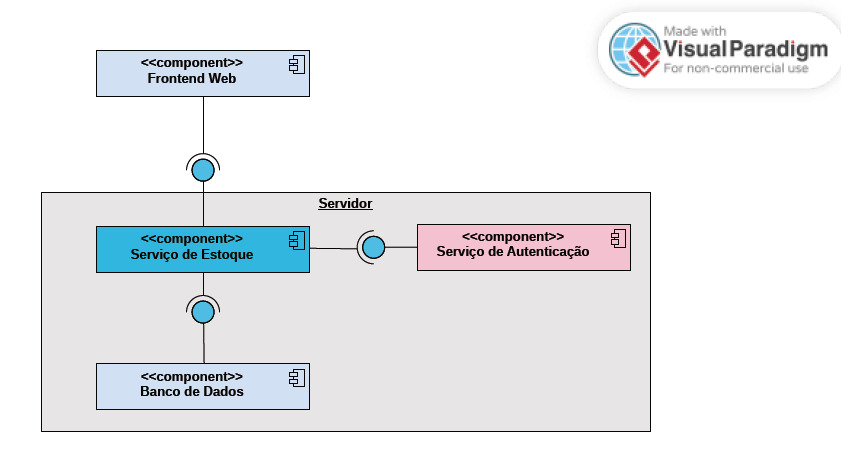
\includegraphics[width=1.0\textwidth]{Figuras/Componentes.png}


\subsubsection{Diagrama de Implantação}


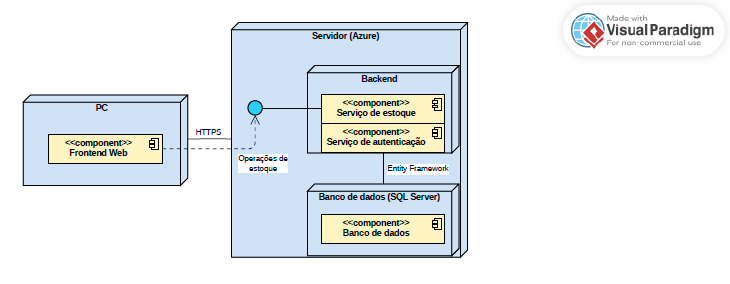
\includegraphics[width=1.0\textwidth]{Figuras/Implantação.png}



\section{Tecnologias}

Esta seção apresenta as principais tecnologias utilizadas no desenvolvimento do sistema, organizadas em categorias como front-end, back-end, banco de dados e infraestrutura. A escolha de cada tecnologia considerou fatores como desempenho, escalabilidade, familiaridade da equipe e compatibilidade com os requisitos do projeto.

\subsection{Front-end}

\begin{itemize}

   \item \textbf{Razor Views}: Arquivos .cshtml que utilizam a engine Razor do ASP.NET para gerar páginas HTML dinâmicas. Essa abordagem permite mesclar código C\# com marcação HTML de forma fluida, facilitando a renderização de conteúdo no lado do servidor e a reutilização de componentes visuais \cite{Razor}.

   \item \textbf{HTML, CSS e JavaScript}: Tecnologias fundamentais para a construção da camada de apresentação do sistema. O HTML estrutura o conteúdo das páginas, o CSS define o estilo visual e o JavaScript adiciona interatividade ao front-end \cite{FrontEnd}.

   \item \textbf{Bootstrap}: Framework front-end baseado em HTML, CSS e JS que oferece componentes prontos e responsivos, facilitando a criação de interfaces modernas, padronizadas e adaptáveis a diferentes dispositivos \cite{Bootstrap}.

   \item \textbf{jQuery}: Biblioteca JavaScript que simplifica a manipulação do DOM, o tratamento de eventos e requisições AJAX. Foi utilizada para agilizar o desenvolvimento de funcionalidades interativas no front-end da aplicação \cite{JQuery}.

\end{itemize}


\subsection{Back-end}

\begin{itemize}

  \item \textbf{C\# com ASP.NET MVC}: Linguagem e framework utilizados na construção do back-end da aplicação, seguindo o padrão arquitetural Model-View-Controller (MVC), que organiza o código de forma modular, separando lógica de negócios, visualização e controle \cite{AspNet2025}.

  \item \textbf{Entity Framework com LINQ}: Conjunto de tecnologias para acesso a dados em .NET. O Entity Framework permite o mapeamento objeto-relacional (ORM), e o LINQ facilita a realização de consultas ao banco de dados de forma legível e integrada ao C\# \cite{EfCore}.

  \item \textbf{ASP.NET Identity}: Sistema de autenticação e controle de acesso da Microsoft utilizado para gerenciar usuários, perfis e permissões de forma segura e integrada ao projeto \cite{Identity}.

  \item \textbf{JJMasterData}: Ferramenta de administração e modelagem de dados que permite a criação dinâmica de formulários e telas de cadastro com base nas entidades do sistema, otimizando o desenvolvimento da interface administrativa \cite{JJMasterdata}.

\end{itemize}

\subsection{Banco de Dados}

\begin{itemize}
    \item \textbf{Microsoft SQL Server}: O Microsoft SQL Server é um sistema de gerenciamento de banco de dados relacional (RDBMS) robusto e amplamente utilizado no mercado, responsável pelo armazenamento seguro das informações da aplicação \cite{SqlServer2025}.


\end{itemize}

\subsection{Infraestrutura}

\begin{itemize}
    \item \textbf{Microsoft Azure}: Plataforma de computação em nuvem utilizada para hospedar a aplicação e seus serviços relacionados. A utilização do Azure proporciona escalabilidade, segurança e alta disponibilidade \cite{Azure2025}. O Azure está sendo utilizado como plataforma principal para a hospedagem de todos os componentes do sistema, abrangendo o banco de dados, o back-end e o front-end.
\end{itemize}



\section{Testes e Manutenção}
Com a evolução da tecnologia, diversas práticas foram desenvolvidas visando um melhor desenvolvimento e manutenção de um projeto. Desde o início do processo de criação de um sistema, questões como escalabilidade, manutenibilidade e usabilidade devem ser consideradas para garantir a longevidade e qualidade do software.

\subsection{Manutenção do Sistema}

A manutenção de software é um processo essencial que ocorre após a implantação da aplicação, seu objetivo é garantir o funcionamento contínuo e eficiente do sistema. Durante o desenvolvimento deste projeto, foram realizadas manutenções de diferentes tipos:

\begin{itemize}
    \item \textbf{Manutenção Corretiva}: correção de falhas no uso do sistema, foram encontradas algumas ações do sistema em inconformidade com as regras de negócio estabelecidas, algumas inconsistências nos formulários. Também foram identificadas algumas chamadas incorretas no código C\#  
    \item \textbf{Manutenção Evolutiva}: conforme se deu o desenvolvimento, notou-se que algumas outras necessidades surgiram, como mudanças em campos e fluxos do sistema, como por exemplo o campo de observação da movimentação.
    \item \textbf{Manutenção Adaptativa}: atualizações para garantir compatibilidade com novas versões de bibliotecas e frameworks utilizados, como o Bootstrap e componentes do ASP.NET. Além de portabilidades que permitem a compatibilidade com o uso do site por celulares, como a tela de login.
    \item \textbf{Manutenção Preventiva}: otimização de consultas do banco de dados, revisões e refatorações do código fonte e técnicas de proteção de rotas e requisições.
\end{itemize}

Durante todo o processo de manutenção também foi usado em larga escala o versionamento via Git, essencial para o controle de todas as mudanças do projeto. O versionamento com o registro de correções e da evolução do sistema, salvo no histórico de commits do GitHub, foi de grande importância para o desenvolvimento em equipe.

O conjunto dessas ações contribuiu para a estabilidade, escalabilidade e segurança geral do sistema, garantindo assim uma maior satisfação dos Stakeholders.

\subsection{Plano de Testes}

A execução de testes é fundamental para o bom desenvolvimento de uma aplicação, eles devem ser continuamente realizados ao longo de toda construção dos processos de um sistema e também após a sua implementação. A testagem permite uma verificação precisa da qualidade de um software, ajuda a capturar falhas de execução de processos e a atestar que as funcionalidades estão sendo executadas de maneira correta.

\subsubsection{Estratégia de Testes}

A estratégia de testes adotada neste projeto foi centrada em testes manuais exploratórios, realizados ao longo de todo o processo de desenvolvimento. A cada nova funcionalidade implementada, foram conduzidos testes com foco na verificação do comportamento esperado, análise de validações, usabilidade e integridade dos dados.

O foco principal foi validar os seguintes aspectos:
\begin{itemize}
    \item Navegação entre telas e fluxos do sistema.
    \item Validação de formulários com campos obrigatórios e regras de negócio.
    \item Conferência do correto salvamento, atualização e exclusão de dados no banco de dados.
    \item Verificação de mensagens de erro e alertas ao usuário.
\end{itemize}

Como parte da organização, os testes foram documentados por meio de registros no GitHub, vinculando as falhas encontradas aos commits de correção, o que favoreceu o acompanhamento da evolução da qualidade do sistema.

\subsubsection{Escopo dos testes}

Os testes foram realizados dentro de módulos do sistema:

\begin{itemize}
    \item \textbf{Login}: foi testada a obrigatóriedade dos campos de usuário e senha, caso os campos não estejam preenchidos um alerta surgirá, não permitindo o avanço, caso os campos sejam preenchidos o sistema conferirá o usuário e a senha e então permitirá ou não o acesso do usuário.
    \item \textbf{Operações do Banco de Dados}: o cadastro de produtos, movimentações, categorias de produtos, fornecedores e usuários foram testados a fim de garatir que o for feito por meio das telas do sistema de fato criem registros no banco de dados.
    \item \textbf{Comportamento de telas}: o comportamento de botões, navegação, preenchimento de campos e alterações de estados da tela foram testados, alcançando, assim, a melhor experiência possível para o usuário.
\end{itemize}

\newpage

\subsubsection{Casos de teste Funcionais}
\begin{table}[htbp]

\caption{Casos de Teste Funcionais - Módulo de Autenticação}
\begin{tabular}{|p{1cm}|p{1.6cm}|p{3.3cm}|p{2.3cm}|p{3.5cm}|p{3.5cm}|}
\hline
\textbf{ID} & \textbf{Funcio-nalidade} & \textbf{Descrição do Teste} & \textbf{Pré-condições} & \textbf{Passos} & \textbf{Resultado Esperado} \\
\hline
TF001 & Login & Verificar se o sistema permite login com credenciais válidas & Usuário cadastrado no sistema & 
1. Acessar a página de login
2. Inserir nome de usuário válido
3. Inserir senha válida
4. Clicar no botão ``Entrar'' & 
O sistema deve autenticar o usuário e redirecionar para a página inicial do sistema \\
\hline
TF002 & Login & Verificar se o sistema impede login com senha incorreta & Usuário cadastrado no sistema & 
1. Acessar a página de login
2. Inserir nome de usuário válido
3. Inserir senha incorreta
4. Clicar no botão ``Entrar'' & 
O sistema deve exibir mensagem de erro indicando credenciais inválidas \\
\hline
TF003 & Logout & Verificar se o sistema permite que o usuário faça logout & Usuário autenticado no sistema & 
1. Clicar na opção de logout no menu
2. Confirmar a ação se solicitado & 
O sistema deve encerrar a sessão e redirecionar para a página de login \\
\hline
\end{tabular}
\legend{Fonte: Elaborado pelos autores}
\end{table}

\FloatBarrier

\begin{table}[htbp]

\caption{Casos de Teste Funcionais - Módulo de Cadastro de Produtos}
\begin{tabular}{|p{1cm}|p{1.7cm}|p{3.2cm}|p{2.1cm}|p{3.5cm}|p{3.5cm}|}
\hline
\textbf{ID} & \textbf{Funcio-nalidade} & \textbf{Descrição do Teste} & \textbf{Pré-condições} & \textbf{Passos} & \textbf{Resultado Esperado} \\
\hline
TF004 & Cadastro de Produto & Verificar se o sistema permite cadastrar um novo produto com dados válidos & Usuário autenticado com permissões de cadastro & 
1. Acessar o módulo de cadastro de produtos
2. Clicar em ``Novo Produto''
3. Preencher todos os campos obrigatórios
4. Clicar em ``Salvar'' & 
O sistema deve cadastrar o produto e exibir mensagem de sucesso \\
\hline
TF005 & Cadastro de Produto & Verificar se o sistema impede cadastro de produto com código duplicado & Produto já cadastrado no sistema & 
1. Acessar o módulo de cadastro de produtos
2. Clicar em ``Novo Produto''
3. Inserir código já existente
4. Preencher demais campos
5. Clicar em ``Salvar'' & 
O sistema deve exibir mensagem de erro indicando que o código já existe \\
\hline
TF006 & Edição de Produto & Verificar se o sistema permite editar dados de um produto existente & Produto cadastrado no sistema & 
1. Acessar o módulo de produtos
2. Localizar o produto desejado
3. Clicar em ``Editar''
4. Modificar campos desejados
5. Clicar em ``Salvar'' & 
O sistema deve atualizar os dados do produto e exibir mensagem de sucesso \\
\hline
\end{tabular}
\legend{Fonte: Elaborado pelos autores}
\end{table}

\FloatBarrier

\begin{table}[htbp]

\caption{Casos de Teste Funcionais - Módulo de Movimentação de Estoque}
\begin{tabular}{|p{1cm}|p{1.7cm}|p{3.3cm}|p{2.2cm}|p{3.5cm}|p{3.5cm}|}
\hline
\textbf{ID} & \textbf{Funcio-nalidade} & \textbf{Descrição do Teste} & \textbf{Pré-condições} & \textbf{Passos} & \textbf{Resultado Esperado} \\
\hline
TF007 & Entrada de Estoque & Verificar se o sistema registra corretamente a entrada de produtos no estoque & Produto cadastrado no sistema & 
1. Acessar o módulo de movimentação
2. Selecionar ``Entrada de Estoque''
3. Selecionar o produto
4. Informar quantidade
5. Informar data e fornecedor
6. Clicar em ``Registrar'' & 
O sistema deve registrar a entrada e atualizar o saldo do produto \\
\hline
TF008 & Saída de Estoque & Verificar se o sistema registra corretamente a saída de produtos do estoque & Produto cadastrado com saldo disponível & 
1. Acessar o módulo de movimentação
2. Selecionar ``Saída de Estoque''
3. Selecionar o produto
4. Informar quantidade (menor que o saldo)
5. Informar data e destino
6. Clicar em ``Registrar'' & 
O sistema deve registrar a saída e atualizar o saldo do produto \\
\hline
TF009 & Saída de Estoque & Verificar se o sistema impede saída maior que o saldo disponível & Produto cadastrado com saldo disponível & 
1. Acessar o módulo de movimentação
2. Selecionar ``Saída de Estoque''
3. Selecionar o produto
4. Informar quantidade maior que o saldo
5. Informar data e destino
6. Clicar em ``Registrar'' & 
O sistema deve exibir mensagem de erro indicando saldo insuficiente \\
\hline
\end{tabular}
\legend{Fonte: Elaborado pelos autores}
\end{table}

\FloatBarrier

\begin{table}[htbp]

\caption{Casos de Teste Funcionais - Módulo de Relatórios}
\begin{tabular}{|p{1cm}|p{1.5cm}|p{3.2cm}|p{2.1cm}|p{3.5cm}|p{3.5cm}|}
\hline
\textbf{ID} & \textbf{Funcio-nalidade} & \textbf{Descrição do Teste} & \textbf{Pré-condições} & \textbf{Passos} & \textbf{Resultado Esperado} \\
\hline
TF010 & Relatório de Saldo & Verificar se o sistema gera relatório de saldo atual de estoque & Produtos cadastrados com movimentações & 
1. Acessar o módulo de relatórios
2. Selecionar ``Relatório de Saldo''
3. Definir filtros (opcional)
4. Clicar em ``Gerar'' & 
O sistema deve exibir relatório com saldo atual de todos os produtos \\
\hline
TF011 & Relatório de Movimentações & Verificar se o sistema gera relatório de movimentações por período & Movimentações registradas no sistema & 
1. Acessar o módulo de relatórios
2. Selecionar ``Relatório de Movimentações''
3. Definir período
4. Clicar em ``Gerar'' & 
O sistema deve exibir relatório com todas as movimentações do período \\
\hline
\end{tabular}
\legend{Fonte: Elaborado pelos autores}
\end{table}

\FloatBarrier
\subsubsection{Casos de teste não Funcionais}
\FloatBarrier
\begin{table}[htbp]
\centering
\caption{Casos de Teste Não Funcionais - Usabilidade}
\begin{tabular}{|p{1.3cm}|p{3.3cm}|p{3.5cm}|p{2.5cm}|p{4.5cm}|}
\hline
\textbf{ID} & \textbf{Descrição} & \textbf{Critérios de Aceitação} & \textbf{Ferramentas} & \textbf{Resultado Esperado} \\
\hline
TNF009 & Facilidade de uso para novos usuários & Usuários sem treinamento devem conseguir realizar tarefas básicas em até 5 minutos & Teste com usuários reais e cronômetro & Novos usuários devem conseguir realizar operações básicas sem necessidade de treinamento extensivo \\
\hline
TNF010 & Clareza das mensagens de erro & Mensagens de erro devem ser claras e indicar como resolver o problema & Avaliação qualitativa com usuários & As mensagens de erro devem ser compreensíveis e fornecer orientações para resolução \\
\hline
TNF011 & Responsividade em dispositivos móveis & Interface deve se adaptar corretamente a diferentes tamanhos de tela & Teste em diferentes dispositivos ou simuladores & A interface deve ser utilizável e visualmente adequada em smartphones, tablets e desktops \\
\hline
TNF012 & Acessibilidade & Sistema deve atender aos requisitos básicos de acessibilidade  & Ferramentas de análise de acessibilidade & O sistema deve ser utilizável por pessoas com deficiências motoras \\
\hline
\end{tabular}
\legend{Fonte: Elaborado pelos autores}
\end{table}

\begin{table}[htbp]
\centering
\caption{Casos de Teste Não Funcionais - Desempenho}
\begin{tabular}{|p{1.3cm}|p{3.3cm}|p{3.5cm}|p{2.5cm}|p{4.5cm}|}
\hline
\textbf{ID} & \textbf{Descrição} & \textbf{Critérios de Aceitação} & \textbf{Ferramentas} & \textbf{Resultado Esperado} \\
\hline
TNF001 & Tempo de resposta para consulta de produtos & Tempo de resposta deve ser menor que 2 segundos para até 100 produtos & Cronômetro & O sistema deve responder às consultas de produtos dentro do limite de tempo estabelecido, mesmo com um grande volume de dados \\
\hline
TNF002 & Tempo de geração de relatório de movimentações & Relatório com até 1000 registros deve ser gerado em menos de 5 segundos & Cronômetro  & O sistema deve gerar relatórios de movimentação dentro do limite de tempo estabelecido, mesmo com grande volume de dados \\
\hline
TNF003 & Capacidade de processamento simultâneo & Sistema deve suportar até 20 usuários simultâneos sem degradação de desempenho &  ferramenta similar de teste de carga & O sistema deve manter o tempo de resposta aceitável mesmo com múltiplos usuários realizando operações simultaneamente \\
\hline
TNF004 & Tempo de carregamento inicial da aplicação & A aplicação deve carregar completamente em menos de 5 segundos em conexão & Cronômetro  & A interface do usuário deve estar completamente carregada e operacional dentro do limite de tempo estabelecido \\
\hline
\end{tabular}
\legend{Fonte: Elaborado pelos autores}
\end{table}



\section{Segurança, Privacidade, Legislação}

Este tópico é dedicado a explicar sobre as questões de segurança e legislação relevantes para o projeto.

\subsection{Critérios de Segurança e Privacidade}

O sistema de gerenciamento de estoque foi projetado com critérios de segurança e privacidade para garantir a integridade das informações e proteger os dados dos usuários. As principais medidas adotadas no projeto incluem:

\begin{itemize}
    \item \textbf{Autenticação e Autorização:} O acesso ao sistema é controlado por meio de autenticação de usuários, utilizando o \textit{ASP.NET Identity}. Cada usuário precisa estar autenticado para acessar funcionalidades sensíveis, como cadastro de produtos, movimentação de estoque ou relatórios.

    \item \textbf{Criptografia de Senhas:} As senhas dos usuários são armazenadas de forma criptografada (hash) no banco de dados, conforme práticas recomendadas pelo \textit{Entity Framework}.

    \item \textbf{Boas Práticas de Privacidade:} Os dados pessoais dos usuários, como nome e e-mail, são utilizados apenas para fins de autenticação e gerenciamento interno, e não são compartilhados com terceiros.
\end{itemize}

\subsection{Legislação}

A  Lei Geral de Proteção de Dados (LGPD - Lei nº 13.709/2018) garante transparencia diante ao uso de dados pessoais garantindo que os dados coletados sejam utilizados exclusivamente para fins de autenticação, autorização e controle de acesso ao sistema. Sendo assim, o sistema segue as diretrizes da LGPD, adotando medidas técnicas e administrativas adequadas para proteger os dados pessoais contra acessos não autorizados, perda ou vazamento. 

Além da LGPD, o sistema também considera princípios estabelecidos no Marco Civil da Internet (Lei nº 12.965/2014), que estabelece garantias, direitos e deveres para o uso da internet no Brasil.




\section{Modelo de Banco de Dados}

O modelo de banco de dados é responsável por organizar e estruturar as informações utilizadas no sistema, garantindo integridade, consistência e facilidade no acesso aos dados. Nesta seção, são apresentados o Modelo Entidade-Relacionamento (MER), o Diagrama Entidade-Relacionamento (DER) e o Dicionário de Dados. O MER e o DER representam graficamente as entidades, atributos e relacionamentos do sistema, enquanto o dicionário de dados descreve detalhadamente cada campo presente no banco, incluindo tipo, tamanho e função. O modelo foi projetado para gerenciar de forma eficiente o controle de estoque, permitindo registrar entradas, saídas, usuários, produtos, fornecedores e categorias.

\subsection{Modelo Entidade Relacionamento}

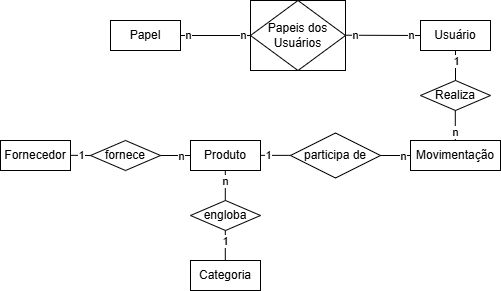
\includegraphics[width=1.0\textwidth]{Figuras/MERestoque.png}


\subsection{Diagrama Entidade Relacionamento}

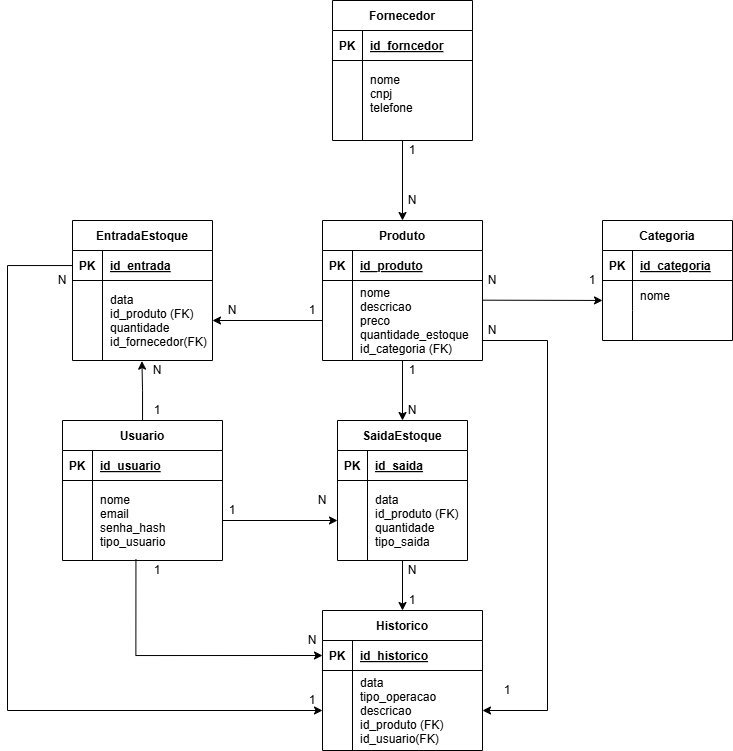
\includegraphics[width=1.0\textwidth]{Figuras/DERestoque.png}


% coloca o dicionário de dados?  \subsection{Dicionário de Dados}

\section{Cronograma}

\subsection{Cronograma de Atividades – Primeiro Semestre}

O desenvolvimento do sistema de gerenciamento de estoque será realizado ao longo de dois semestres letivos, estando o presente cronograma correspondente às atividades planejadas para o primeiro semestre. Neste período inicial, o foco principal está na fundamentação e planejamento do projeto, bem como na construção da prova de conceito e definição do escopo mínimo viável.

\begin{itemize}

\item No início do semestre, tem-se a fase de Desenvolvimento do Tema (Entrega do marco dia 08/04/2025), que contempla a escolha do assunto central do projeto e a definição do parceiro institucional. Essa etapa foca no levantamento detalhado dos requisitos (funcionais e não funcionais) e na análise de viabilidade do sistema proposto.

\item Posteriormente, desenvolve-se a fase de Desenho da Aplicação (Entrega do marco dia 29/04/2025), com foco na estruturação técnica da solução. Aqui, são entregues o projeto do banco de dados (MER e DER), os diagramas de arquitetura (UML) e a modelagem dos processos de negócio (AS IS e TO BE).

\item A seguir, passa-se à etapa de Prova de Conceito (Entrega do marco dia 20/05/2025), na qual se realiza a escolha das tecnologias mais adequadas. O resultado é o desenvolvimento dos protótipos iniciais de interface, dos scripts de criação do banco de dados e o início da implementação do back-end do sistema.

\item Por fim, inicia-se a fase da Criação do MVP (Produto Mínimo Viável) (Entrega do marco dia 17/06/2025). Essa etapa inclui a definição clara do problema e das prioridades, delimitando o escopo da aplicação com suas restrições. O produto final é a identificação das funcionalidades mínimas essenciais e das integrações necessárias.

\item Paralelamente, é elaborada a fase de Análise e Documentação (Entrega do marco dia 18/07/2025), cujo objetivo é consolidar os dados obtidos. Esta seção inclui a elaboração da introdução, revisão da literatura, gestão do projeto e análise de viabilidade financeira, encerrando com as considerações finais sobre o processo.
\end{itemize}

% \subsection{Análise da duração do projeto}

\chapter{Viabilidade Financeira}

\section{Custos}

A Tabela 2 apresenta uma análise pormenorizada e multidimensional dos custos de desenvolvimento, detalhando o investimento fundamental em mão de obra, que representa o principal ativo do projeto. Sua estrutura, ao desagregar os custos por perfil técnico — como desenvolvedores sênior, analistas de qualidade e gestores de projeto —, permite identificar com precisão onde o capital está sendo alocado. A cada uma dessas funções é atribuída uma estimativa de esforço em horas de trabalho, fornecendo uma base quantitativa para o planejamento. A metodologia de cálculo, que se destaca pela transparência e objetividade, consiste na multiplicação do esforço previsto pela taxa horária específica de cada especialista, garantindo uma apuração fiel à realidade do mercado e evitando as distorções de estimativas genéricas.

Esta abordagem, portanto, transcende um simples levantamento numérico. Ela não só oferece clareza sobre os custos inerentes a cada fase do desenvolvimento, mas, ao ser projetada sobre a duração total de 9 meses, transforma-se em uma poderosa ferramenta de gestão estratégica e preditiva. A projeção temporal permite uma análise aprofundada da distribuição dos custos mensais e globais, oferecendo previsibilidade e permitindo a antecipação de picos de investimento. Com isso, a gestão pode mitigar riscos financeiros, como desvios orçamentários, antes que se concretizem.

Consequentemente, a tabela constitui um pilar para um planejamento financeiro robusto, que justifica o orçamento perante stakeholders e estabelece uma linha de base para o controle rigoroso das despesas, viabilizando a alocação otimizada de recursos e assegurando a sustentabilidade operacional do projeto.

\begin{table}[hbtp]
    \centering
    \caption{Detalhamento dos Custos de Desenvolvimento.}
    \label{tab:custos_desenvolvimento_simples}
    \begin{tabular}{|l|c|c|c|c|c|}
        \hline
        \textbf{Função} & \textbf{Quant.} & \textbf{Horas/Dia} & \textbf{Dias} & \textbf{Valor/Hora (R\$)} & \textbf{Total (R\$)} \\
        \hline
        Product Owner (PO)    & 1 & 6 & 180 & 25,00 & 27.000,00 \\
        \hline
        DBA (MySQL/Azure)     & 1 & 6 & 180 & 22,00 & 23.760,00 \\
        \hline
        Desenvolvedor Front-end & 1 & 6 & 180 & 18,00 & 19.440,00 \\
        \hline
        Desenvolvedor Back-end  & 2 & 6 & 180 & 20,00 & 43.200,00 \\
        \hline
        Especialista em SI    & 1 & 6 & 180 & 23,00 & 24.840,00 \\
        \hline
        QA (Testes)           & 1 & 6 & 180 & 16,00 & 17.280,00 \\
        \hline
        \textbf{Total} & \textbf{7} & - & - & - & \textbf{155.520,00} \\
        \hline
    \end{tabular}
    Duração do projeto: 9 meses (180 dias úteis). Custo MO mensal: R\$ 17.280,00.
\fonte{Elaborado pelos autores.}
\end{table}

Na tabela 3 é representada a estrutura mensal da empresa, detalhando os custos associados às instalações, equipamentos e serviços de TI. No item 2.1, destacam-se os gastos com aluguel de espaço e mobiliário, totalizando 0 reais por mês. Já no item 2.2, referente à aquisição de equipamentos, observa-se que não há custos neste momento. No entanto, no item 2.3, estão listados os custos mensais de serviços de TI.

\begin{table}[hbtp]
\centering
\caption{Estrutura Mensal da Empresa.}
\label{tab:estrutura_mensal}
\begin{tabular}{lcr}
\toprule
\textbf{Item} & \textbf{Quantidade} & \textbf{Valor (R\$)} \\
\midrule
\multicolumn{3}{l}{\textbf{2. Estrutura da empresa (mensal)}} \\
\addlinespace % Adiciona um pequeno espaço vertical
\quad 2.1. Instalações - Aluguel & - & 0,00 \\
\addlinespace
\multicolumn{3}{l}{\quad 2.2. Equipamentos (TI e Outros)} \\
\qquad - Computadores/notebooks & 0 & 0,00 \\
\qquad - Servidores proprietários & 0 & 0,00 \\
\qquad - Outros (mobiliário, etc.) & 0 & 0,00 \\
\addlinespace
\multicolumn{3}{l}{\quad 2.3. Serviços de TI} \\
\qquad - Ferramentas de desenvolvimento & - & 0,00 \\
\qquad - Hospedagem e banco de dados & - &99,83 \\
\midrule
\textbf{Total mensal} & & \textbf{R\$ 99,83} \\
\bottomrule
\end{tabular}
\fonte{Elaborado pelos autores.}
\end{table}


\section{Cenário realista}
Na figura 9 no cenário realista, em que o ponto de equilíbrio é alcançado em cerca de 15 meses, considerando um investimento inicial de R\$ 155.520 e receita mensal média de R\$ 30.600.
\begin{center}
  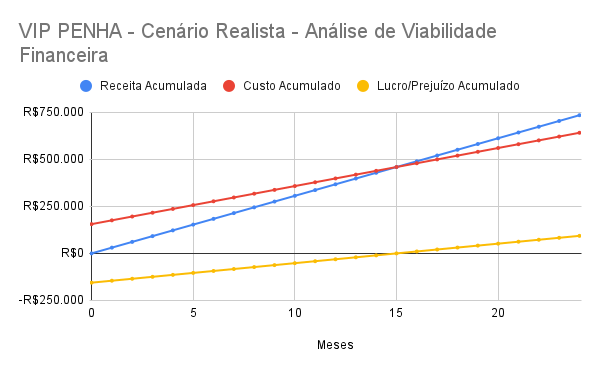
\includegraphics[width=0.9\textwidth]{Figuras/CenarioRealista.png}
\end{center}

\section{Cenários otimista}
Na figura 10 no cenário otimista, o ponto de equilíbrio é alcançado em cerca de 9 meses, com receitas 25\% acima do projetado.
\begin{center}
  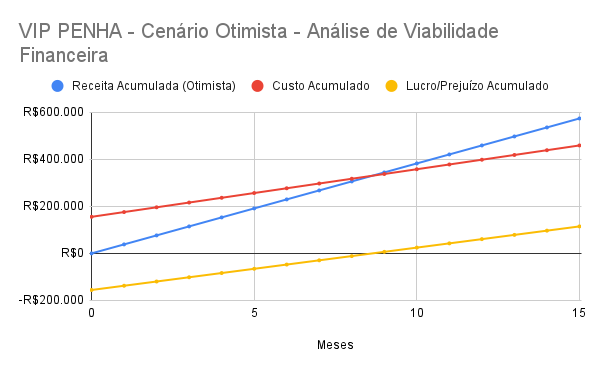
\includegraphics[width=0.9\textwidth]{Figuras/CenarioOtimista.png}
\end{center}

\section{Cenários pessimista}
Na figura 11 no cenário pessimista, o ponto de equilíbrio é alcançado em cerca de 37 meses, com receitas 20\% abaixo do projetado.
\begin{center}
  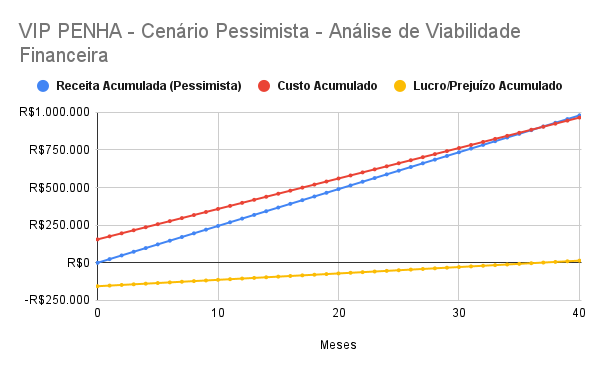
\includegraphics[width=0.9\textwidth]{Figuras/CenarioPessimista.png}
\end{center}

\chapter{Considerações Finais}
Ao longo do desenvolvimento deste projeto, que visa a criação de um sistema de controle de estoque para um estabelecimento comercial, foi possível constatar de soluções tecnológicas para otimizar processos e garantir a eficiência operacional em ambientes comerciais. A iniciativa de desenvolver este sistema surgiu da necessidade de modernizar a gestão  em um cenário de mercado cada vez mais competitivo.
O sistema proposto representa uma ferramenta estratégica para a loja, Vip Penha permitindo o cadastro detalhado de produtos, o controle preciso de entradas e saídas de mercadorias, e a geração de relatórios gerenciais. Essas funcionalidades são necesarias para reduzir erros manuais, tempo dedicado à organização do estoque e, consequentemente, aprimorar a tomada de decisões. A implementação de uma metodologia ágil, como o Kanban, foi de grande ajuda para a organização do projeto.
Conclui-se que a aplicação deste sistema resulta em uma melhora substancial na gestão do estoque do estabelecimento, contribuindo para a redução de perdas, a otimização do fluxo de trabalho e por consequência ganhos econômicos. Além disso, este projeto demonstra o potencial das tecnologias da informação para resolver desafios práticos do cotidiano de empreendimentos. A contínua evolução e aprimoramento de tais sistemas é essencial para que empreendimentos e empresas   possam manter sua competitividade e prosperar no mercado atual.

%\section{Dificuldades, escolhas e descartes}
%Durante o desenvolvimento do projeto, enfrentamos desafios inerentes à complexidade de um sistema de controle de estoque, nas etapas iniciais de modelagem e arquitetura. Uma das primeiras dificuldades surgiu na elaboração do Diagrama de Entidade-Relacionamento (DER) e do diagrama de componentes. A primeira tentativa de construir esses diagramas revelou a necessidade de um aprofundamento maior das relações entre as entidades do sistema e na definição clara dos módulos e suas interações. Este processo inicial de tentativa foi crucial para refinar a visão e garantir uma base sólida para o desenvolvimento 
%Uma escolha crucial foi unificar o histórico de movimentações de produtos em uma única tabela, em vez de usar tabelas separadas para entradas e saídas. Essa decisão visou simplificar e otimizar a consulta e a unificação dos dados, melhorando o desempenho e a consistência.

% ---
% Apêndices
% ----------------------------------------------------------

% ---
% Inicia os apêndices
% ---
\begin{apendicesenv}

% Imprime uma página indicando o início dos apêndices
%\partapendices

% ----------------------------------------------------------
\chapter{Mapeamento de Processos}
% ----------------------------------------------------------
\section{Processo AS IS e TO BE}

\subsection{Processo AS IS (Situação Atual)}

\subsection*{Descrição Geral}
A loja faz controle de estoque manualmente, por anotações em papel feitas pelo dono.

\subsection*{Etapas do Processo}

\begin{enumerate}
    \item \textbf{Recebimento de produtos (entrada)}: O dono recebe os produtos de fornecedores. Ele anota em um caderno: nome do produto, quantidade recebida, data e fornecedor.
    
    \item \textbf{Venda de produtos (saída)}: Ao vender um produto, o dono anota à mão no mesmo caderno: nome do produto, quantidade vendida, data e valor da venda.
    
    \item \textbf{Controle de estoque}: O dono consulta o caderno para verificar a quantidade de produtos disponíveis. Não há atualização automática; o controle depende da leitura e interpretação das anotações.
    
    \item \textbf{Relatório mensal}: O dono folheia o caderno, soma manualmente as entradas e saídas e tenta fazer um resumo no final do mês. Processo demorado e sujeito a erros.
\end{enumerate}

\subsection*{Problemas Identificados}

\begin{itemize}
    \item Alto risco de erro humano.
    \item Dificuldade em rastrear movimentações específicas.
    \item Falta de relatórios precisos.
    \item Perda ou danos ao caderno comprometem todo o controle.
    \item Nenhuma visibilidade em tempo real do estoque.
\end{itemize}

\subsection{Processo TO BE (Situação Proposta com Sistema)}

\subsection*{Descrição Geral}
Será implementado um sistema informatizado para registrar entradas, saídas e gerar relatórios mensais automaticamente.

\subsection*{Etapas do Processo com o Sistema}

\begin{enumerate}
    \item \textbf{Recebimento de produtos (entrada)}: O dono ou funcionário acessa o sistema. Registra os produtos recebidos: nome, quantidade, fornecedor, data, nota fiscal. O estoque é atualizado automaticamente.

    \item \textbf{Venda de produtos (saída)}: No momento da venda, o produto é registrado como “vendido” no sistema. O sistema subtrai automaticamente a quantidade vendida do estoque.

    \item \textbf{Controle de estoque}: O sistema exibe em tempo real o estoque disponível de cada item. Alertas de baixo estoque podem ser configurados.

    \item \textbf{Relatório mensal de movimentações}: Ao fim do mês (ou sob demanda), o sistema gera automaticamente um relatório com:
    \begin{itemize}
        \item Total de entradas por produto.
        \item Total de saídas por produto.
        \item Saldo atual.
        \item Produtos mais vendidos.
        \item Histórico por período.
    \end{itemize}
\end{enumerate}

\subsection*{Benefícios Esperados}

\begin{itemize}
    \item Redução de erros manuais.
    \item Facilidade no rastreamento de movimentações.
    \item Economia de tempo.
    \item Maior controle e visibilidade sobre o estoque.
    \item Dados organizados e acessíveis a qualquer momento.
\end{itemize}
% ----------------------------------------------------------
%\lipsum[55-57]

\end{apendicesenv}
% ---
% ----------------------------------------------------------
% Finaliza a parte no bookmark do PDF
% para que se inicie o bookmark na raiz
% e adiciona espaço de parte no Sumário
% ----------------------------------------------------------
\phantompart




% ----------------------------------------------------------
% ELEMENTOS PÓS-TEXTUAIS
% ----------------------------------------------------------
\postextual
% ----------------------------------------------------------

% ----------------------------------------------------------
% Referências bibliográficas
% ----------------------------------------------------------
\bibliographystyle{abntex2-alf}
\bibliography{referencias}

% ----------------------------------------------------------
% Glossário
% ----------------------------------------------------------
%
% Consulte o manual da classe abntex2 para orientações sobre o glossário.
%
%\glossary

% ----------------------------------------------------------

% ----------------------------------------------------------
% Anexos
% ----------------------------------------------------------

% ---
% Inicia os anexos
% ---
%\begin{anexosenv}

% Imprime uma página indicando o início dos anexos
%\partanexos

% ---
%\chapter{exemplo 2}
% ---
%\lipsum[30]

% ---
%\chapter{Cras non urna sed feugiat cum sociis natoque penatibus et magnis dis
%parturient montes nascetur ridiculus mus}
% ---

%\lipsum[31]

% ---
%\chapter{exemplo 3}
% ---

%\lipsum[32]

%\end{anexosenv}

%---------------------------------------------------------------------
% INDICE REMISSIVO
%---------------------------------------------------------------------
\phantompart
\printindex
%---------------------------------------------------------------------

\end{document}
